\chapter{Preprocessing}\label{preprocessing}
Before movement patterns between buildings and building-parts can be retrieved, pre-processing of the raw data is required. In this chapter the different pre-processing steps will be described in detail. First section … addresses the initial data filtering. Section … concerns the grouping of records with the same mac address and location that are subsequent in time. Section … describes the filling of the dataset with a ‘world’ location. This enables detection of movement from and to the campus on the building level, and movement from and to the building on building-part level. Finally section … is about the filtering of records of people only passing by a building or building-part.\\

\section{Initial filtering}\label{generalfiltering}
Each record in the wifilog represents the scanning of a certain device at a certain time by a certain access point. In order to detect the movement patterns of these devices between buildings it should be known for each access point in which building it is located. The apname field in the wifilog table includes the building id in which building each scanner is located. However for some access points the apname is given in a different format and as a result their location is unknown. These apnames have in common that they don’t contain the ‘-’ character which is present in all the other apnames. As a result the apnames of which the location is not known can simply be filtered out by checking if a ‘-’ is present in the apname. Two other special cases are present in which the building id in the apname is 1 or 102. These id’s corresponds to the legermuseum and … respectively. As the legermuseum in not located on the campus it was decided to omit this building. For building-part level the general filtering is much easier, as only the records of a single building are of interest. Therefore, the records that don’t have the building id of the particular building can simply be filtered out. 

\section{Grouping of states}\label{grouping}
In order to reduce the data and to be able to filter out records of people only passing by a building, the data needs to be grouped. The overall goal is to identify movement patterns between different buildings or building-parts. As a result records of subsequent states of the same device in the same building or building-part can be grouped together into one single record. Namely, if two subsequent states are at the same location they don’t represent a movement and can thus be grouped. When looking at building level, the mobile of someone who studies the whole day at architecture might have 20 records (states) in the database for that day. This can be reduced to one record (state) that contains the time the device arrived at Architecture and left again. For building-part level the same applies for someone that has multiple subsequent states in the same building-part. To determine whether two records are subsequent in time, and therefore should be grouped together, a threshold for the time gap between two records needs to be defined. It was decided to set the gap threshold for grouping states to 1 hour. The reasoning behind this is that someone who is not scanned for a period of more than 1 hour has likely left the building. However, if someone is away for less than an hour it more likely that that person was just smoking or lunching outside or just disconnected for from the system for a while. \autoref{figure:grouping} gives an example of how the records are grouped on building level for one device for one single day. It should be noted that two states remain at faculty A as the gap between 12:30 and 13:45 is bigger than an hour. In the other other cases the gap is smaller than an hour and the records are grouped together. Only one records is present at faculty B so this record can not be grouped. The grouped records still contain all the information that is required to know that the person moved from faculty A to B to C during the day. 

\begin{figure}[H]
\centering
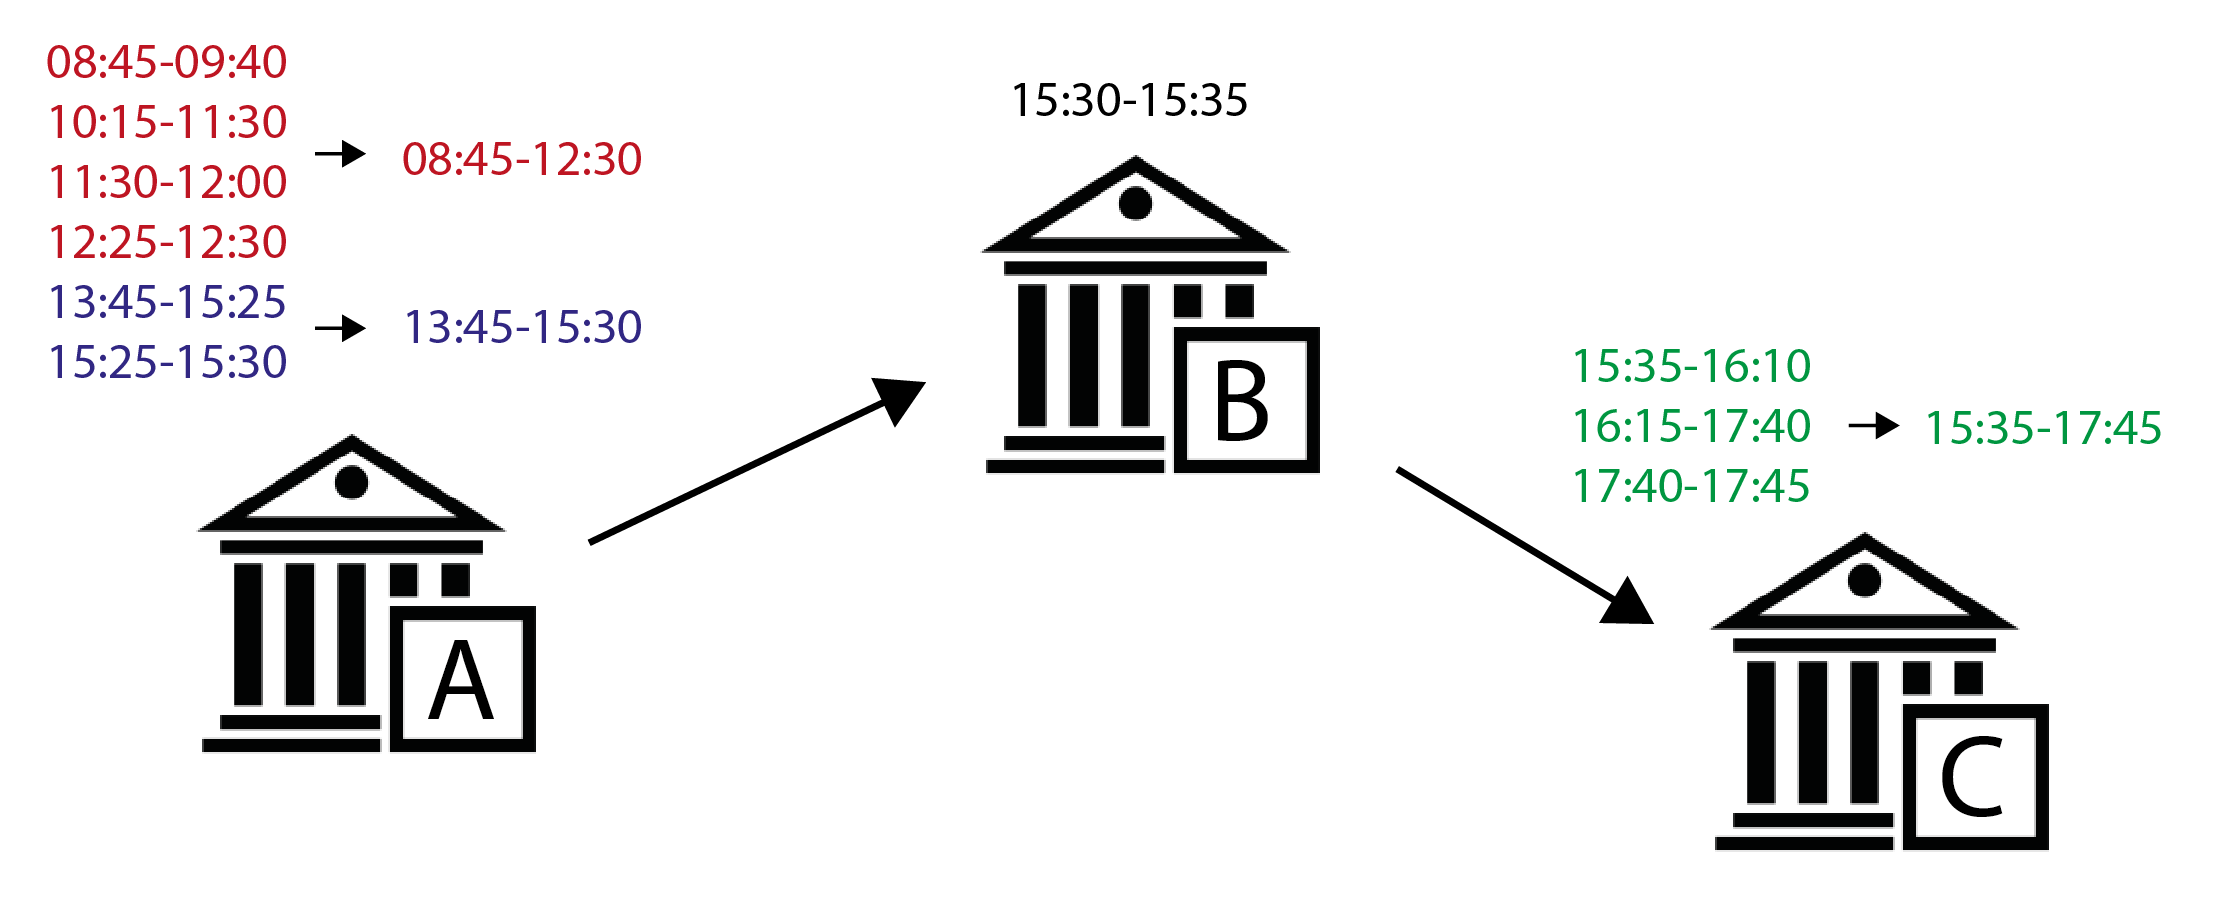
\includegraphics[scale=0.7]{Preprocessing_Grouping}
\captionsetup{justification=centering}
\caption{Grouping}
\label{figure:grouping}
\end{figure}

\section{Adding world state}\label{Adding world}
Because the dataset contains all records of when certain devices are scanned, it also Implicitly stores information on when the device is not located at the campus. These time gaps in which a particular device is not scanned at the campus give information on when the corresponding person is not at the campus. This information is valuable for detecting movement patterns from and to the campus in addition to the movement between buildings at the campus. Considering the fact that many student only visit one faculty each day. It becomes especially clear, that the movement from and to the campus plays an important role in the overall movement pattern of a person. In order to be able to directly derive movement from and to the campus from the dataset, the time gaps present in the data should be stored explicitly. Therefore each time gap larger than an hour is filled with a outside campus or 'world' record. The word 'world' is used to indicate that the device could be located at any place in the world outside the campus during the time spans that it is not scanned at the campus. It should be noted the reason that a device is not connected to one of the access points could also be that the device is simply switched of, in this case however the assumption is made that the device moves off campus. The begin and end time of a world record is defined by the end of the previous record and the start of the next record in time. In case there is no previous or next record the boundaries are defined by the starting time of the whole dataset and the current time. \autoref{figure:world} visualizes the explicit storing of world states that fill time gaps during which a device is not recorded on campus. In can be seen that three 'world' states are added in the example. First during the start of the day before the person goes to faculty A, second during the lunch break, and finally in the end of the day starting from the moment when the person leaves faculty C. Storing these world states explicitly enriches the data as much more movement can be defined. The grouping of records described in \autoref{grouping} and adding of a world state are complementary. If the gap between two states is smaller than an hour they are grouped if the gap is bigger than an hour a world state is inserted. For the building-part level the insertion of world states works exactly the same. In this case however the world represent the outside building area instead of outside campus area.

\begin{figure}[H]
\centering
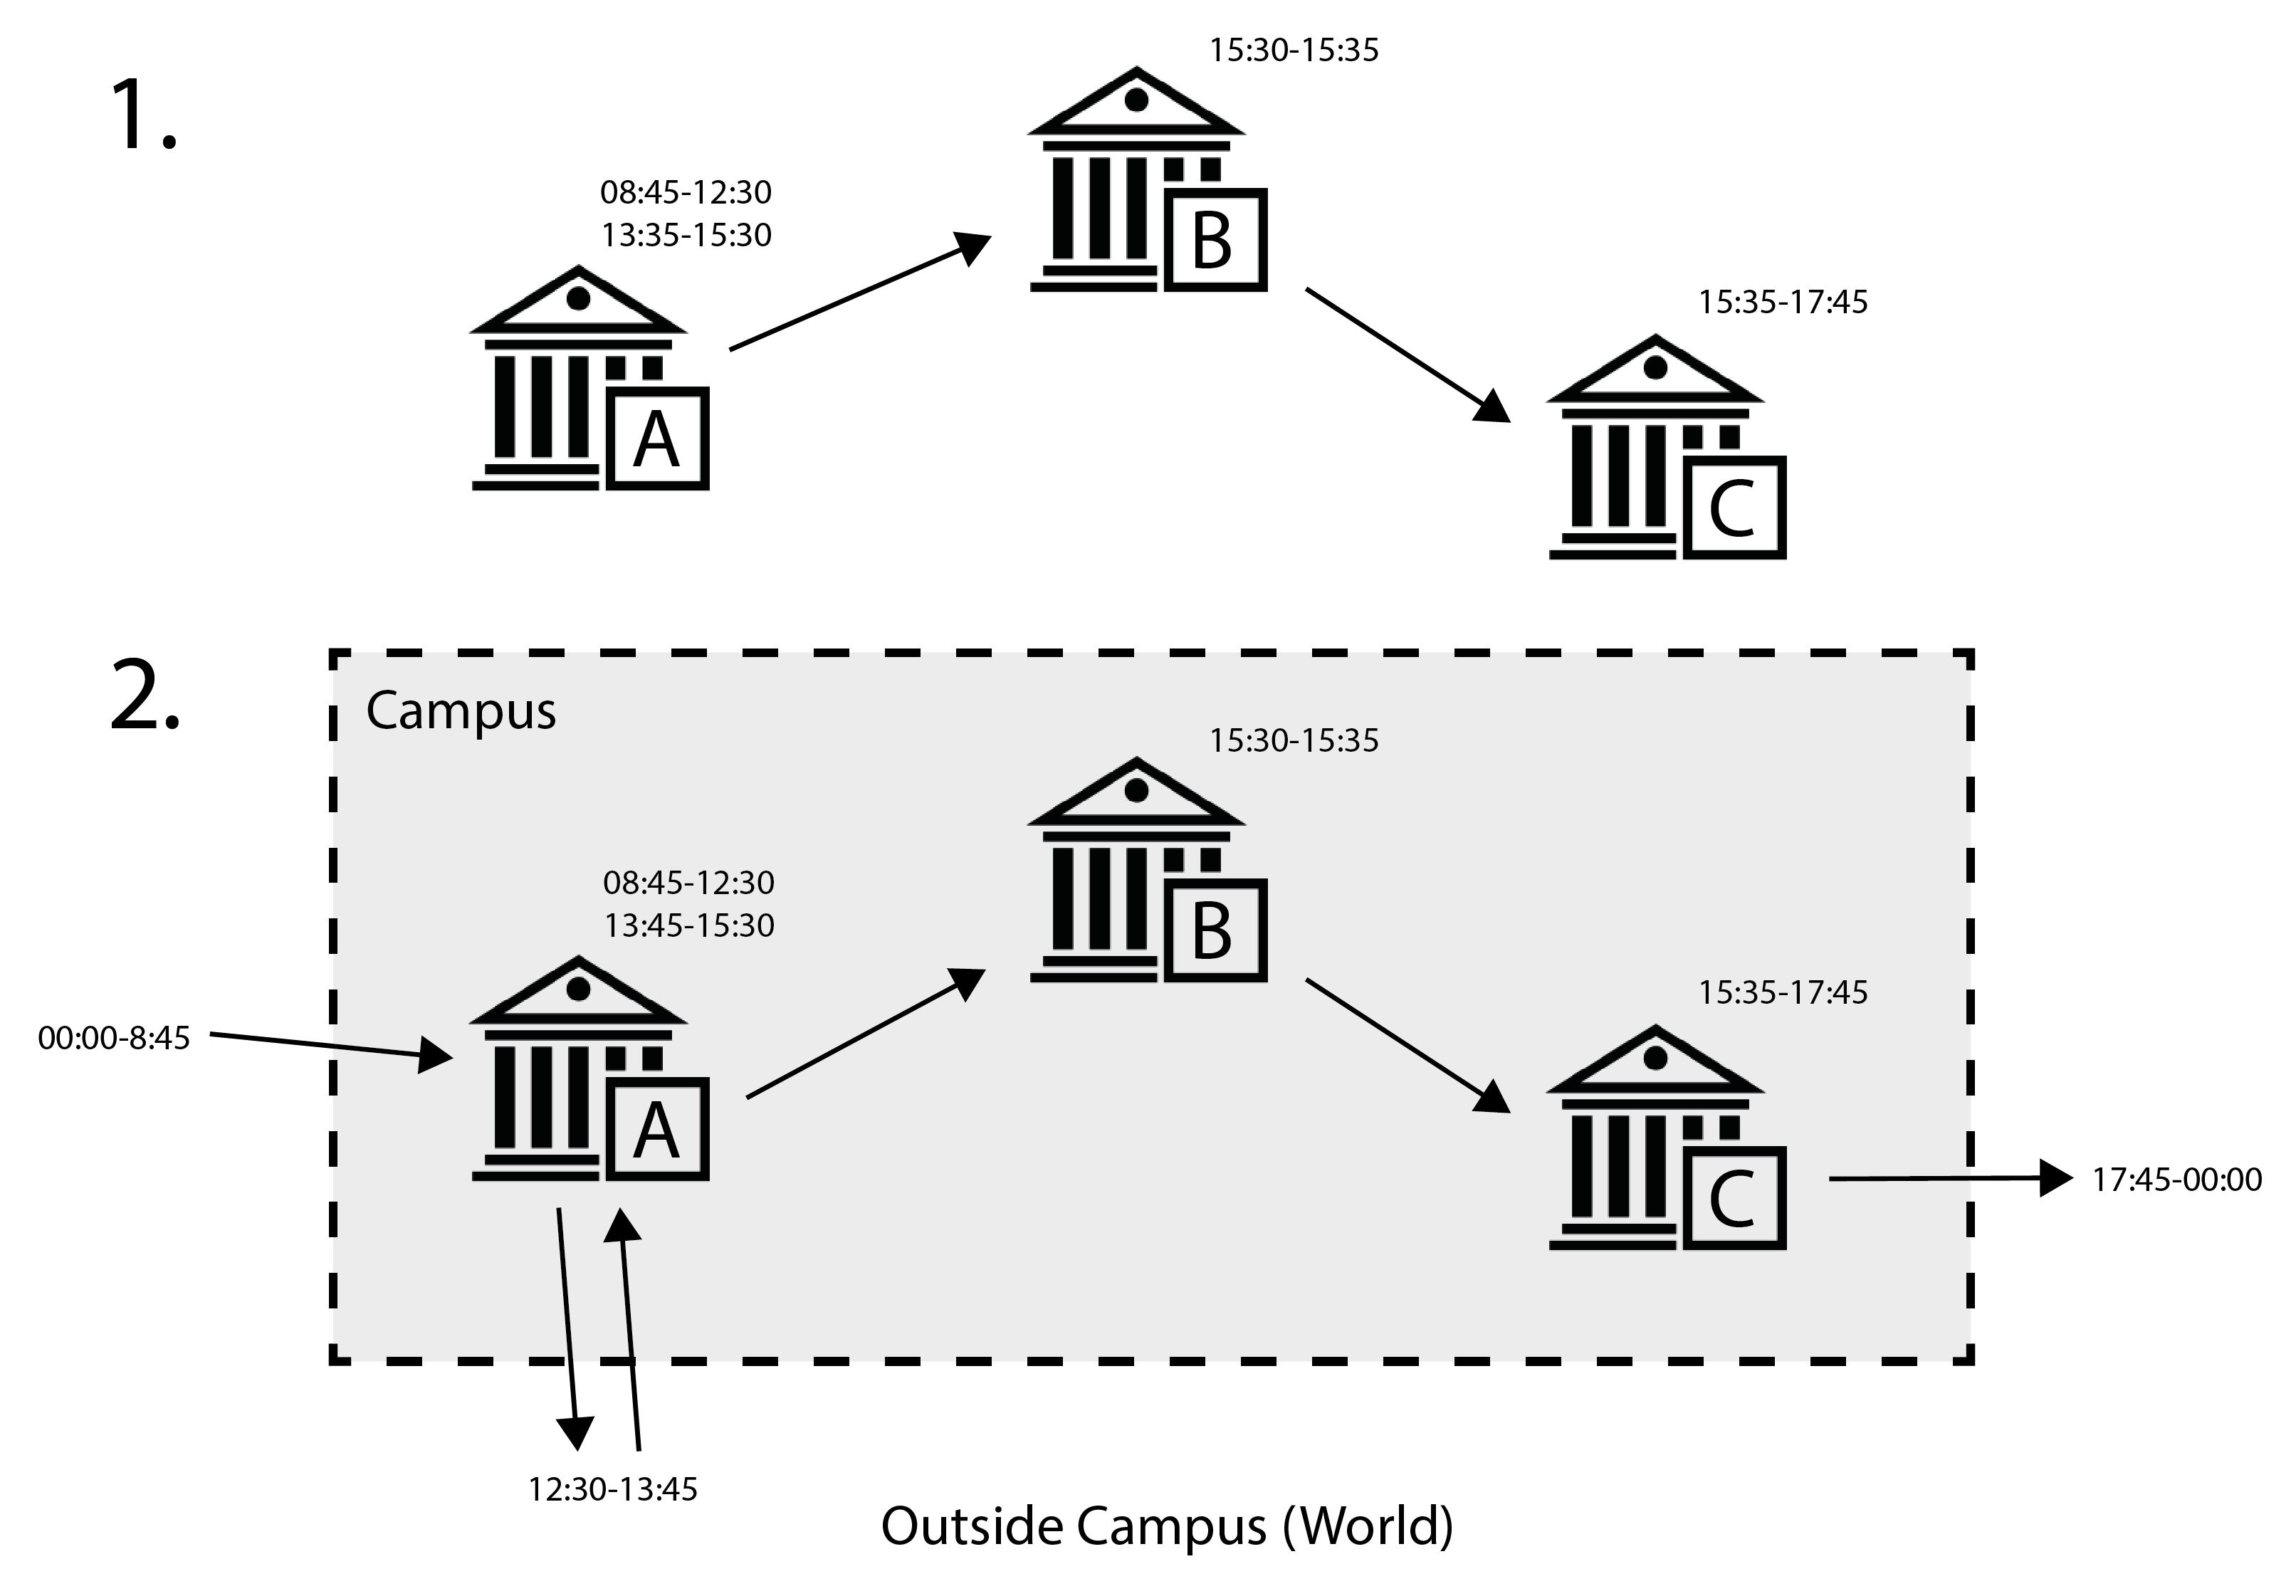
\includegraphics[scale=0.57]{Preprocessing_World}
\captionsetup{justification=centering}
\caption{Adding World}
\label{figure:world}
\end{figure}

\section{Passing by}\label{passing by}
For the detection of movement patterns between buildings, records of people that only pass by a building without actually visiting it should be excluded. The reason for this is that records of people only passing by a building could result in misinterpretation of the movement patterns. This is illustrated by the example in \autoref{figure:passing by}. In this case faculty B is located on the route from faculty A to faculty C. Therefore it is likely that people moving from faculty A to faculty C are picked up by a scanner located at faculty B. The eduroam system records all devices at intervals of approximately 5 minutes as explained in \autoref{datadescription}. Such a recording by the eduroam system can happen during the short time period that the device, which is on its way from faculty A to C, is connected at faculty B. This will result in records of approximately 5 minutes at faculty B, whilst the person has not been inside faculty B. As the movement is the change between two states, the movement to faculty C will origin from faculty B. Someone that is not aware of the 'passing by' problem might conclude that people from faculty B often go to faculty C. In reality however, people from faculty A go often to faculty C. By filtering out the records of people only passing by buildings the correct movement can be visualized (see \autoref{figure:passing by} bottom). It should be noted that filtering out 'passing by' records can only be done after the grouping process. The reason for this is that 5-minute records that would individually be classified as someone passing by might be grouped together into one record with a longer duration. After grouping the combined record is not classified as someone who passes by anymore. Furthermore it should be noted that the filtering of 'passing by' records occurs after filling the data with 'world' states. The reason for this is that a passing by event does mean that the device was located on the campus. The world records are meant to represent the time the device is not on the campus. Filtering passing by events works exactly the same for the building-part level. If a person only passes by a particular building-part without staying in it, it is filtered out. For building-parts this filtering is especially important as the route from one building-part to another often leads through several other building-parts. 

\begin{figure}[H]
\centering
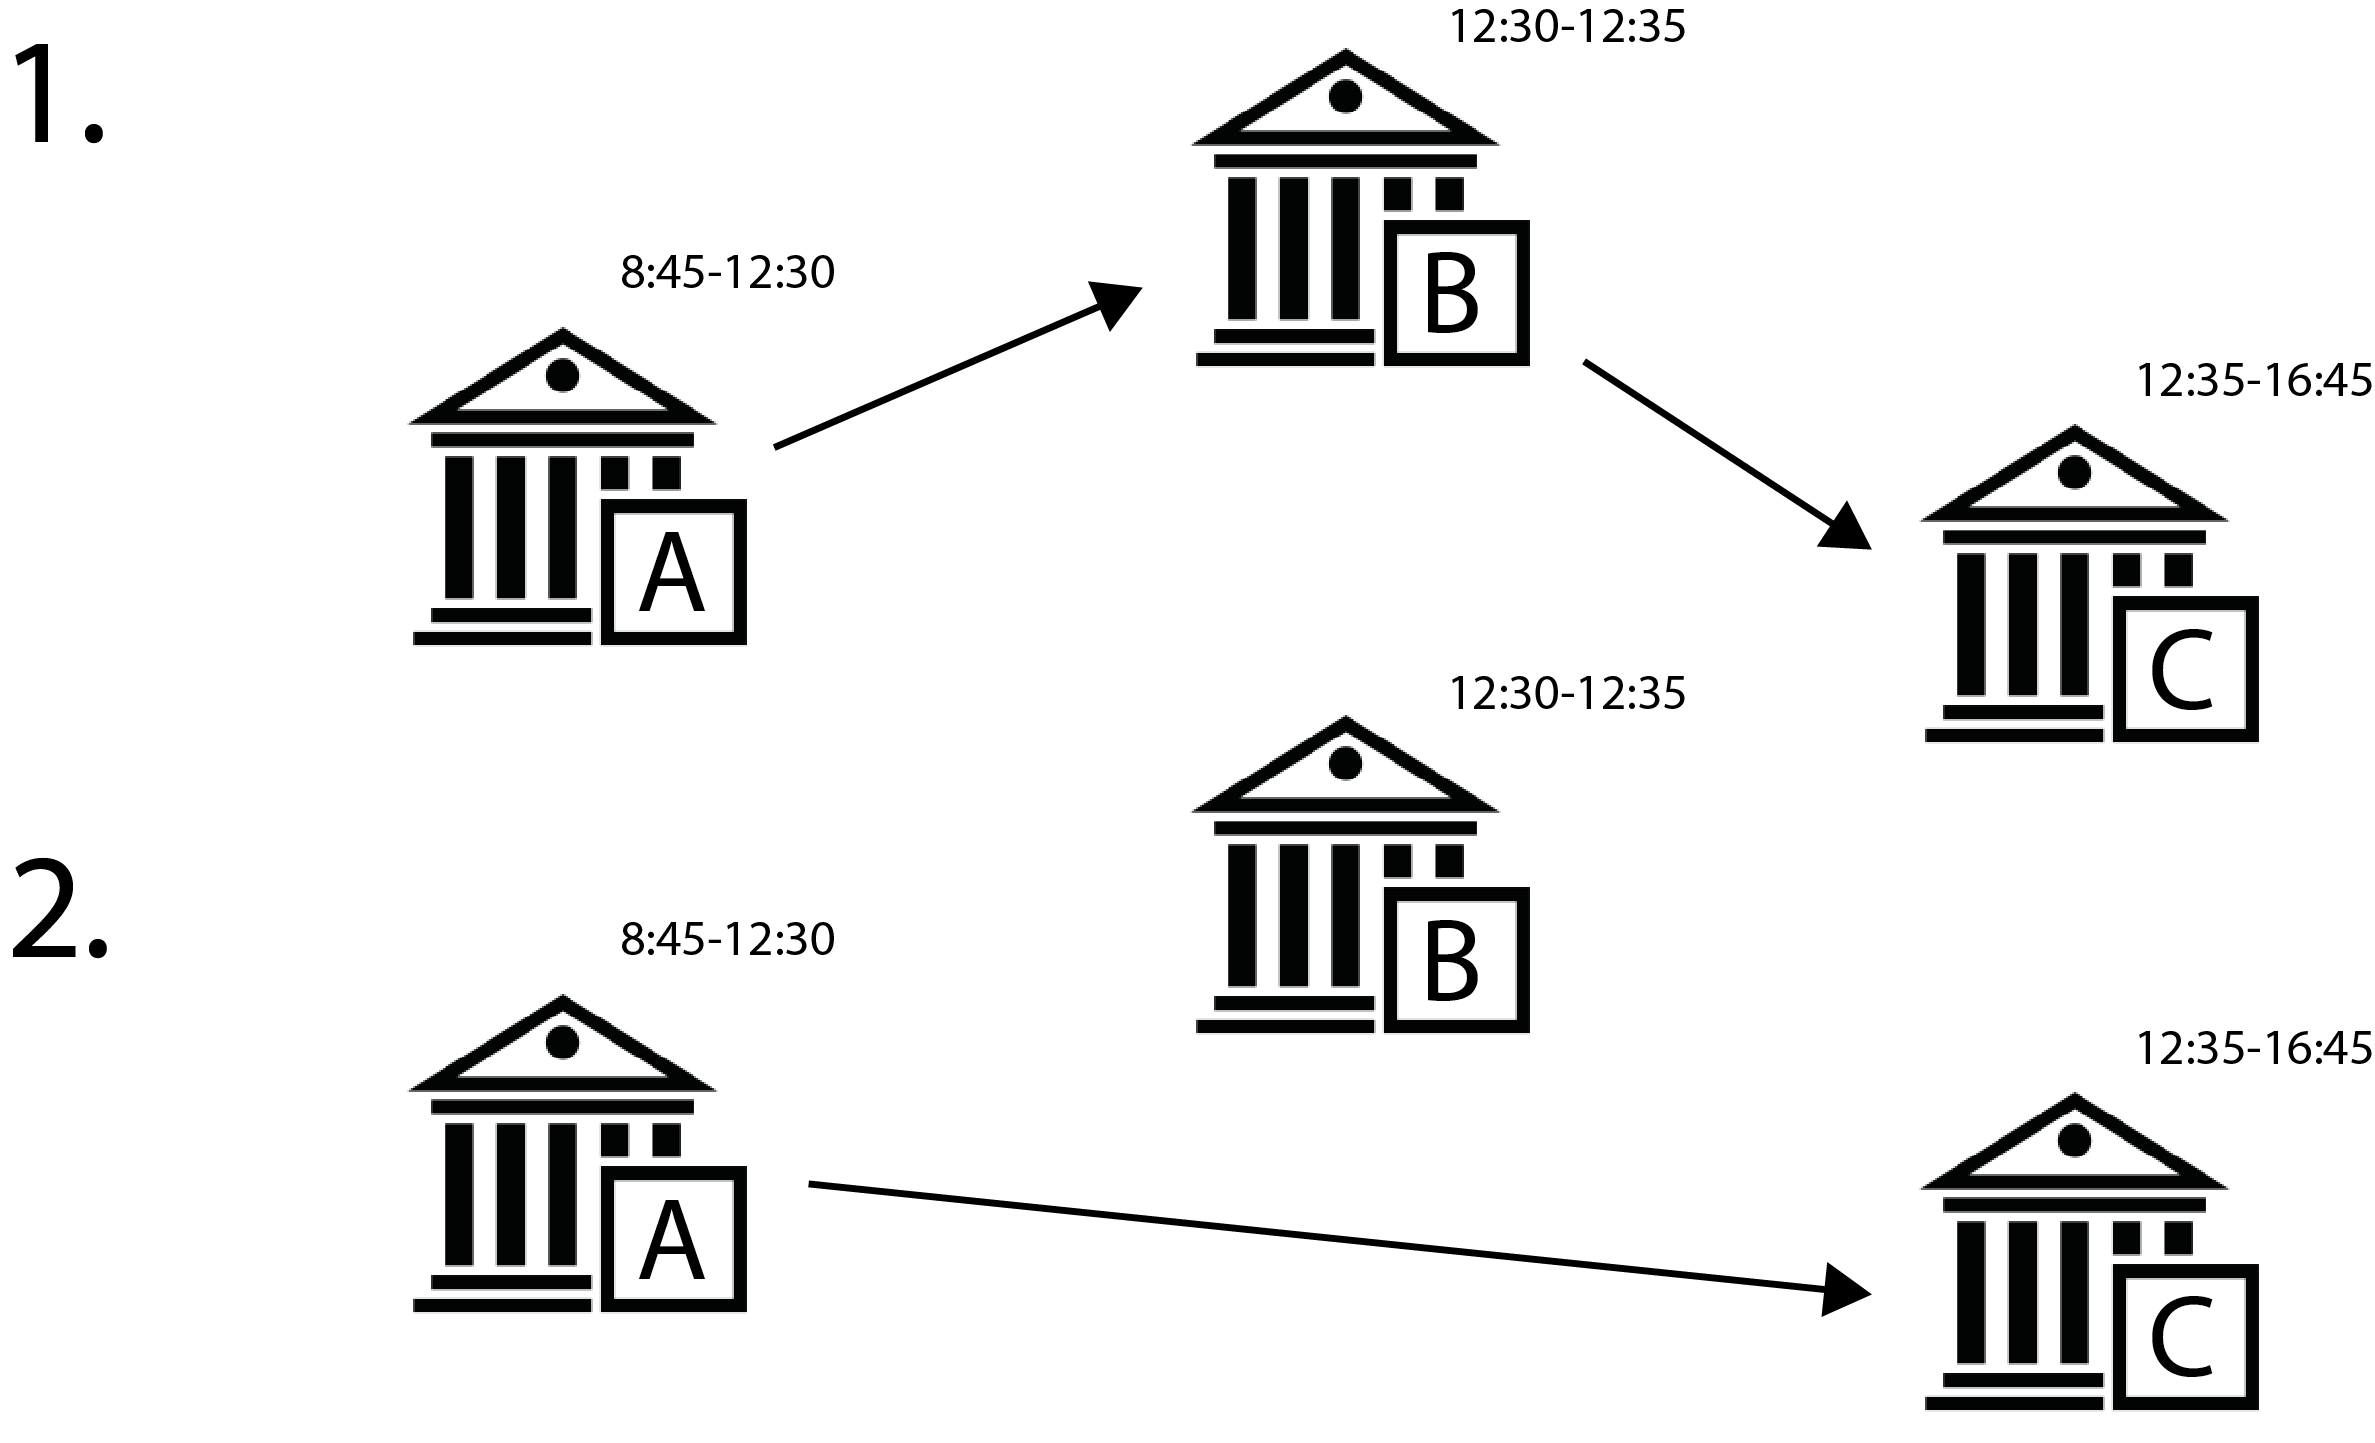
\includegraphics[scale=0.7]{Preprocessing_PassingBy}
\captionsetup{justification=centering}
\caption{Passing by}
\label{figure:passing by}
\end{figure}

\section{Implementation}
The filling (world), grouping and filtering (passing by) steps described above are implemented in an integrated way. The Pseudocode for the implementation for building level is shown in \autoref{figure:pseudocode}, for building-part level the implementation is exactly the same only grouping is done for building-parts instead of buildings. As can be seen in the code there is communication with the database at several points. The table from which the records are retrieved for each mac address is already processed as described in the general filtering section. Furthermore the format of the table is slightly different compared to the initial wifilog. The session duration is exchanged for an end time column which is derived by adding the session duration to the asstime (start time of a record).

\begin{figure}[H]
\centering
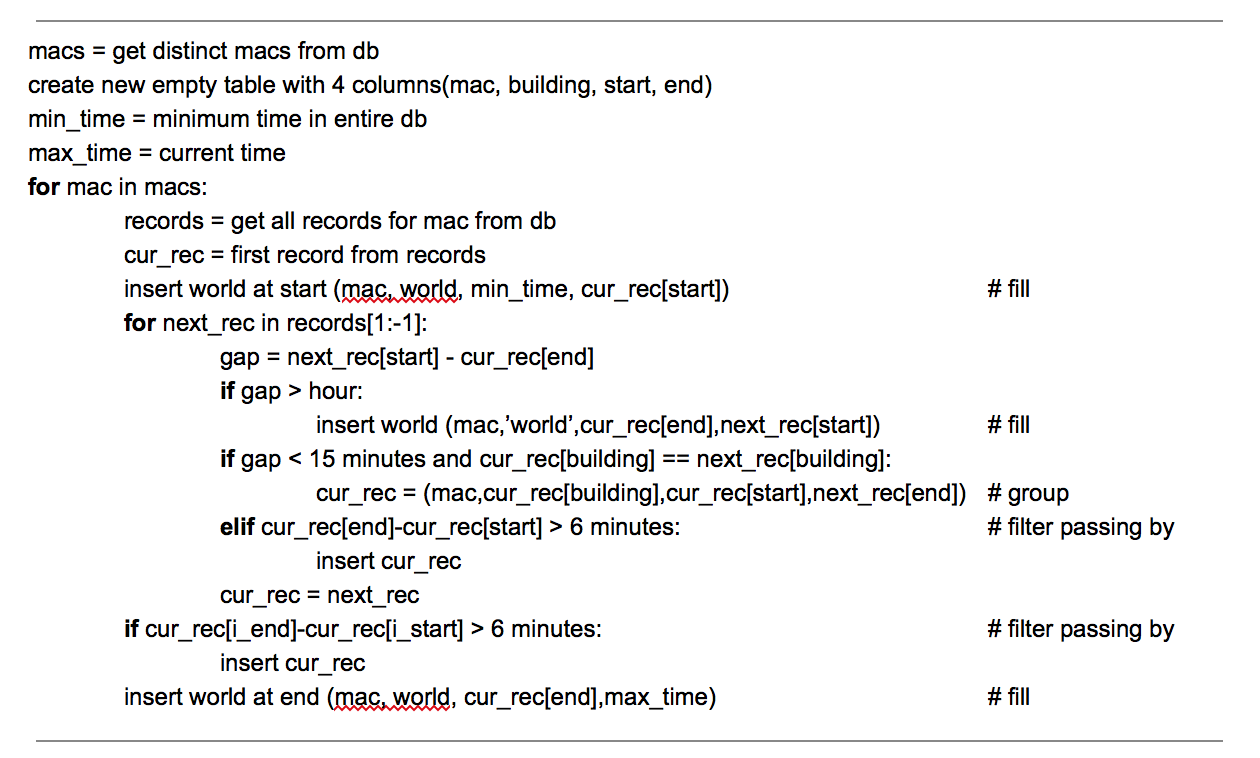
\includegraphics[scale=0.5]{pseudocode.png}
\captionsetup{justification=centering}
\caption{Pseudocode preprocessing}
\label{figure:pseudocode}
\end{figure}

\autoref{figure:Preprocessing} shows an example of the records of one device over a time span of one day during the different pre-processing steps. From the raw data it can be seen that this person spends most of the day in building B. The person is scanned once at building A before he arrives in the morning and after what is likely to be his lunch break. The last two hours the person is scanned in building C. After filling three world records are added, at the beginning of the day, during the lunch break, and at the end of the day. The grouped records show that the subsequent scans in building B and C are grouped together. Finally the scans at building A are removed from the dataset as they are likely to indicate passing by events. 

\begin{figure}[H]
\centering
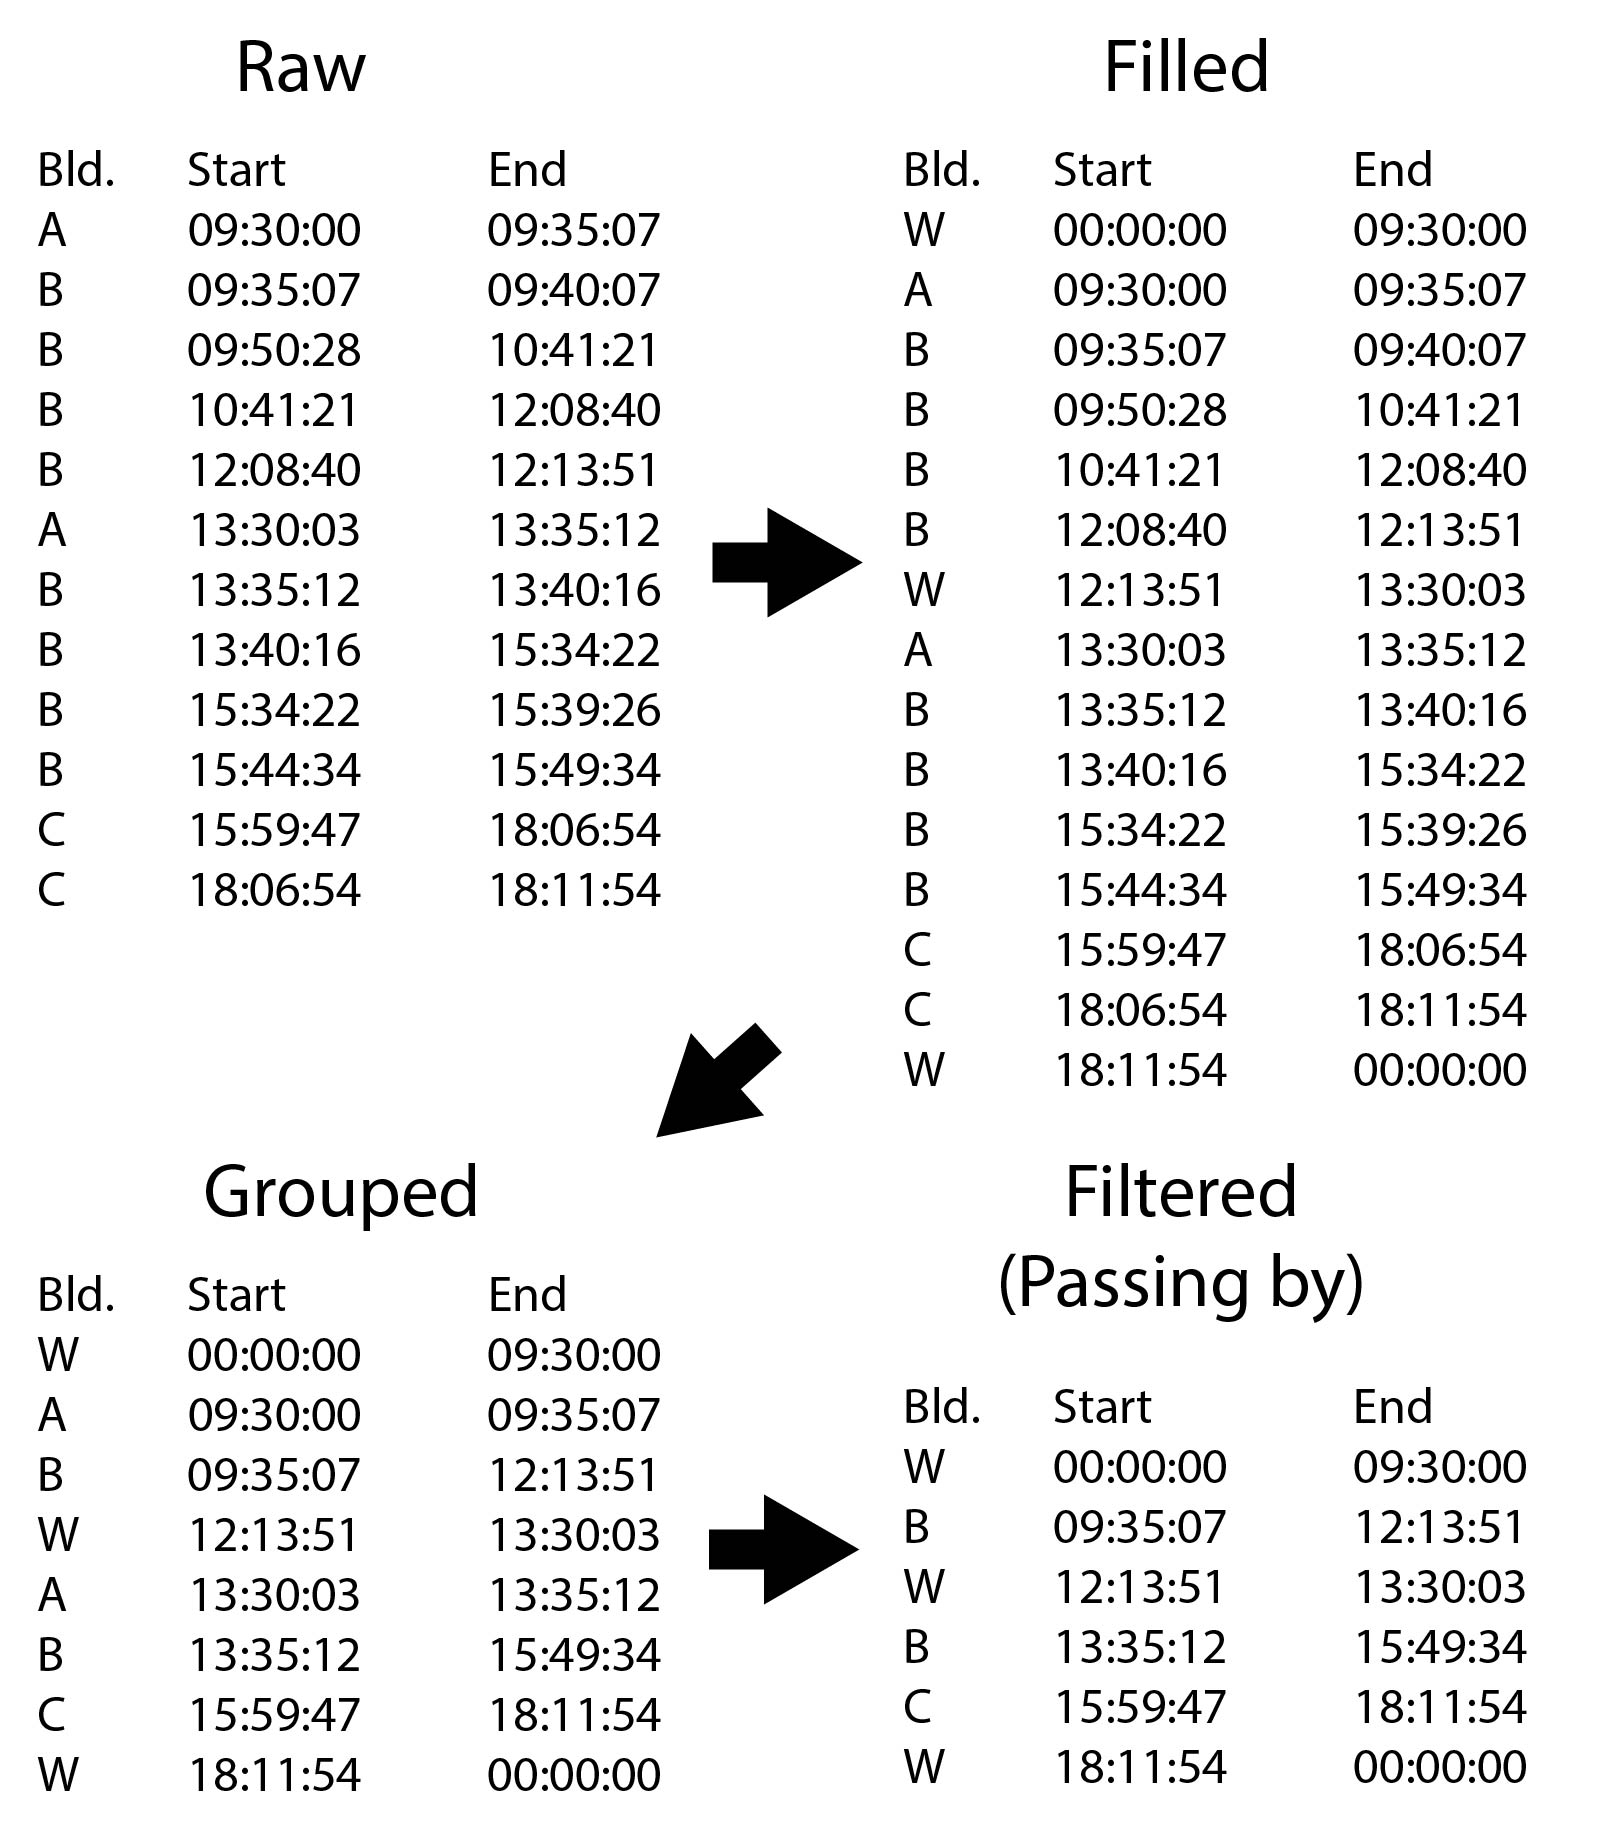
\includegraphics[scale=0.2]{PreProcessing-01.jpg}
\captionsetup{justification=centering}
\caption{Preprocessing}
\label{figure:Preprocessing}
\end{figure}


\section{Apname vs maploc}
The data in the table 'wifilog' contains information about the location of the Access Point (AP) in two columns. The first one is the column 'apname', which is a string with the symbolic name of the AP, for example 'A-08-G-010'. The two numbers in the second part of the string, in this case '08', represent the building number. This building number can be linked to a location in the world. 
The second column which contains information about location, is the column 'maploc'. This column also contains strings, which look as follows:

System Campus $>$ [buildingid] $>$ [specific location]'. An example of such a string is 'System Campus $>$ 21-BTUD $>$ 1e verdieping'. In such a string, the middle part can be linked to a building, so to a real-world location. 
But there are some other values for maploc, which can less clearly be linked to a real-world location. Such a value is 'Root Area', it is unclear what this value means and it contains no information about a building or area it might be in. This makes it impossible to link it to a location in the world. Then there is the value 'Unknown', a value that indicates that there was no name attached to the Access Point that user was connected to. Again in this case, it is impossible to link this value to a real-world location. 

As both 'Root Area' and 'Unknown' are in the minority of records, they could be left out of the queries. But for some records, the column 'apname' did provide information about the location, while the 'maploc' column value was 'Root Area'. In most of these cases however, the building number, the second part of the string, was a number of length three. But there are no buildings on the TU Delft campus with a building number that high. When consulting Wilko Quack about this, he explained that these building numbers had an arbitrary 1 in front of the building number. So 'A-134-A-001' was not building 134, but building 34, which was an actual building number on the campus. This would mean that using the column 'apname' for getting the building number would mean a higher number of results and therefore a more realistic visualization of the movements. 

Taking the substring of that column and linking it to a building with an actual location is done in two steps. First the whole string is retrieved and with a function in Python the substring is derived. Subsequently, the building id that is the result of this function can be linked to a table in the database which has for every building five columns: buildingid, name, point (as geometry), x (longitude), y (latitude) (see in \autoref{maps}).

\section{Static and mobile devices}\label{Static and mobile devices}

In order to identify the movement patterns and know what entrances and exits are most frequently used even better, we aim to identify dynamic and static devices. In our first approach, we will look at the number of different access points the device is scanned by in time. The distinction between static and dynamic devices is important, because the behaviour, in terms of Wi-Fi tracking, is significantly different. For instance, a static device, such as a laptop, connects with the Wi-Fi network at different moments compared to a dynamic device, such as a mobile phone. The difference will be explained more in detail using the image below. 

Assume a person that carries a static device (laptop) and a dynamic device (mobile phone) enters a building. While being on his way to the destination, the person does not make use of the laptop, thus the laptop is not connected to the Wi-Fi network. On the other hand, the Wi-Fi of the mobile phone is turned on all the time, and connects at the moment the device is on range of the first access point. On the way the mobile phone is scanned by Access Point(AP) 1, 2 and 3. The person connects to the Wi-Fi network with the laptop at the moment it arrives in the room, of which the Wi-Fi is covered by AP 3. This access point scans the laptop for first time after entering the building. The static laptop is distorting the result, due the fact that in this case the entrance access point for the laptop would be AP 3. In order to achieve a more reliable result, the aim is to filter out the static devices.

To identify the static and dynamic devices, we analyze the behaviour of each device. The first approach focuses on the number of (distinct) access points and the session duration. We assume to find differences between them (\autoref{table:staticanddynamic}). 

\begin{table}[H]
\centering
\begin{tabular}{|c|c|c|}
\hline 
 & Session duration & Nr.of access points \\
\hline
Static & long & low \\
\hline
Dynamic & short & high \\
\hline	
\end{tabular}
\captionsetup{justification=centering}
\caption{Difference between static and dynamic devices}
\label{table:staticanddynamic}
\end{table}

We expect that the relation between the distinct access points and the (summed) session duration, called ratio, is going to be useful in making the distinction between static and dynamic devices (\autoref{equation:staticdynamic}).

\begin{equation}\label{equation:staticdynamic}
Ratio = distinct access point / summed session duration
\end{equation}

In this, a small ratio indicates the device is dynamic and a large ratio indicates the device is static. The result shows that the number of devices decreases over ratio(\autoref{figure:staticanddynamic}).
\begin{figure}[H]
\centering
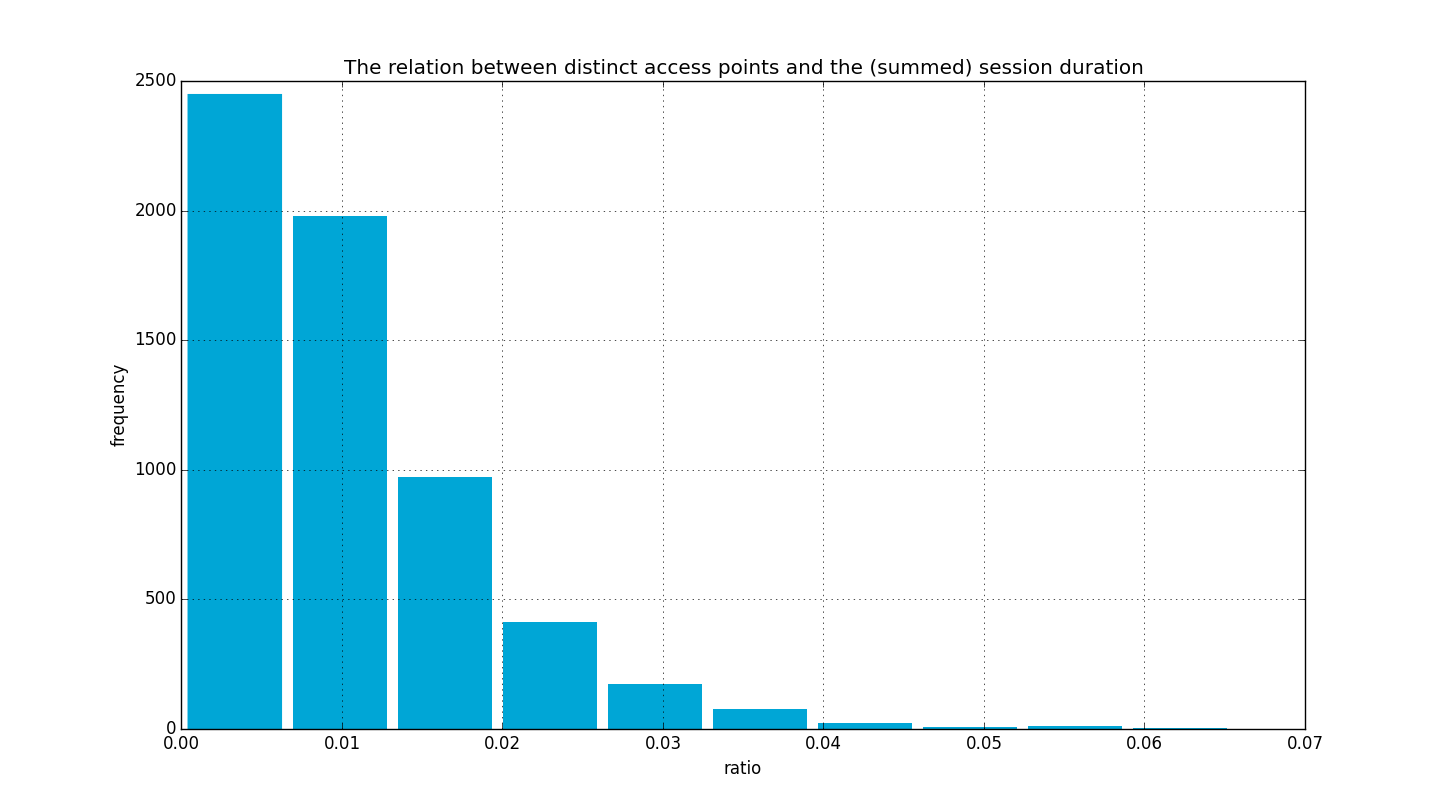
\includegraphics[scale=0.4]{static_vs_dynamic_histogram}
\captionsetup{justification=centering}
\caption{The relation indicating frequency of a radio}
\label{figure:staticanddynamic}
\end{figure}

Because the frequency decreases gradually, there is a fuzzy boundary that separates the static from dynamic devices. Therefore it not (yet) possible to filter out the static devices for further analysis. In order to improve this, the plan is to use the exact number of access points that scanned the device instead of the distinct access points. Also, a closer look will be taken at the session duration, since dynamic devices will have session duration of approximately 5 minutes much more often. 